\documentclass[12pt]{article}

% Fonte com acentos
\usepackage[brazil]{babel} \usepackage[utf8]{inputenc} \usepackage[T1]{fontenc}
\usepackage[lighttt]{lmodern} \usepackage[top=1.4in, bottom=1in, left=1in,
right=1in]{geometry} \usepackage{graphicx} % para adicionar imagem
\usepackage{listings} \usepackage{amsmath} \usepackage{indentfirst}
\usepackage{multicol}

\begin{document}

\setlength{\parskip}{0.2cm}

\title{Análise de código e eficiência do método do Gradiente}

\author{Aryane Ast dos Santos\\ Kevin Katzer}

\date{23 de novembro de 2014}

\maketitle

\tableofcontents

\pagebreak

\section{Introdução}

Este trabalho consiste na análise e otimização da implementação do método do
gradiente apresentado anteriormente. Compara tempo de execução, uso de cache,
memória e Flops entre versões com e sem otimização.

Porém, como a otimização não saiu conforme o planejado, e o desempenho não
melhorou, o trabalho teve que ser entregue sem a análise dos gráficos após a
otimização. Não obstante, os códigos otimizados foram mantidos para avaliação do
professor no momento da apresentação do trabalho.

\section{Verificação de uso de memória com Valgrind}\label{sec:Valgrind}

Ao executar a ferramenta Valgrind para se obter informações sobre vazamento de
memória no programa gradSolver, foi possível observar 5 erros, todos em
contextos diferentes, além de 16 allocações e apenas 2 liberações de memória.

Os resultados da execução do programa são parcialmente apresentados na
figura~\ref{fig:valgrindOut}.

\begin{figure}[htb]
\begin{tt}\noindent
==29599== Command: ./gradSolver -r 5\\
==28949== HEAP SUMMARY:\\
==28949==     in use at exit: 560 bytes in 14 blocks\\
==28949==   total heap usage: 16 allocs, 2 frees, 800 bytes allocated\\
==28949== LEAK SUMMARY:\\
==28949==    definitely lost: 560 bytes in 14 blocks\\
==28949== ERROR SUMMARY: 5 errors from 5 contexts (suppressed: 0 from 0)
\end{tt}\caption{Saída do Valgrind}\label{fig:valgrindOut}
\end{figure}

Aqui o gradSolver foi executado com uma matriz quadrada de ordem 5, porém os
mesmos problemas listados na figura~\ref{fig:valgrindOut} são encontrados em
execuções de matrizes de qualquer dimensão. E de maneira análoga, ao resolver os
problemas apresentados, numa execução com matriz maior, eles ficam também
automaticamente resolvidos.

Para contornar os vazamentos de memória encontrados, foi necessário liberar a
memória dos vetores alocados explicitamente como o vetor x na função main, o
vetor aux em calcGrad e o vetor r de resíduo na função gradSolver. Além disso,
no main, foram adicionados frees para os ponteiros para char das flags do
getopt.

\section{Arquitetura do computador}\label{sec:likwid}

Utilizando a ferramenta likwid-topology, é possível obter as seguintes
informações sobre a arquitetura do computador utilizado para os testes de
performance.

\begin{figure}[ht]\footnotesize
\begin{tt}
\begin{multicols}{2}
CPU type:	AMD Magny Cours processor\\
Hardware Thread Topology\\
Sockets:	4\\
Cores per socket:	8\\
Threads per core:	1\\
Socket 0: ( 0 1 2 3 4 5 6 7 )\\
\\
\\
NUMA Topology\\
NUMA domains: 2\\
Domain 0:\\
Processors: 0 1 2 3 4 5 12 13 14 15 16 17\\
Relative distance to nodes: 10 21\\
Memory: 2403.31MB free of total 24103.8MB\\
\end{multicols}
\begin{multicols}{3}
Cache Topology\\
Level:	1\\
Size:	64 kB\\
Type:	Data cache\\
Associativity:	2\\
Number of sets:	512\\
Cache line size:64\\
Non Inclusive cache\\
Shared among 1 threads\\
Level:	2\\
Size:	512 kB\\
Type:	Unified cache\\
Associativity:	16\\
Number of sets:	512\\
Cache line size:64\\
Non Inclusive cache\\\
Shared among 1 threads\\
\\
Level:	3\\
Size:	5 MB\\
Type:	Unified cache\\
Associativity:	96\\
Number of sets:	512\\
Cache line size:64\\
Non Inclusive cache\\
Shared among 4 threads\\
\end{multicols}
\end{tt}\caption{Saída resumida do likwid-topology}\label{fig:topologyOut}
\end{figure}

Como pode-se notar na figura~\ref{fig:topologyOut}, nas servidoras do DInf, há
uma CPU Magny Cours, fabricada pela AMD, com 4 socket e 32 cores (8 por socket).

Existem 3 níveis de cache, sendo o primeiro (L1) com 64kB de memória, o segundo
(L2) com 512kB e o terceiro (L3) com 5MB. As caches L1 e L2 são separadas em 32
grupos, sendo que cada grupo é destinado a um core diferente, e o último nível
de cache, L3, é separado em 8 grupos, cada grupo destinado a 4 cores.

Há 8 domínios NUMA, e cada domínio correspondendo a uma cache L3. Como apenas o
Socket 0 será usado, apenas o primeiro domínio NUMA é de interesse para análise
de memória disponivel. O domínio 0 possui 16047.3MB de memória RAM, e no momento
de execução do likwid-topology, havia 10269.2MB de memória livre.

Dada a especificação acima, o maior sistema linear passível de ser resolvido
pela arquitetura descrita é aproximadamente 36600, pois, dada a memória RAM
disponível, e sabendo que o programa aloca $n^2 + 3n$ doubles, temos que $64(n^2 +
3n) = 10269.2\times2^{23}$.

\section{Comparação de desempenho geral}\label{sec:desempenhoGeral}

Para a execução dos testes de desempenho, foi utilizada a ferramenta
likwid-pin, que afixa a execução do programa à um core da máquina em uso
dedicado. Mas como a cache L3 continua sendo compartilhada, analisar o
desempenho de diferentes execuções se torna um problema, pois é necessário
minimizar o uso da cache pelos outros programas.  Uma solução encontrada foi
executar o gradSolver em mode single user, porém não foi possível utilizar a
solução com os testes apresentados. Vale notar que no período de testes não
haviam outros usuários logados na máquina.

No gráfico~\ref{fig:execucao}, são mostrados os tempos de execução em segundos,
que foram obtidos com a função timestamp, para matrizes de dimensões 32, 256,
1024 e 2048. Na escala horizontal do gráfico, as diferenças entre as potências
de 2 e $2^n+1$ não aparecem claramente. Os eixos do gráfico estão em escala
logarítmica.

\begin{figure}[htb] \begin{center}
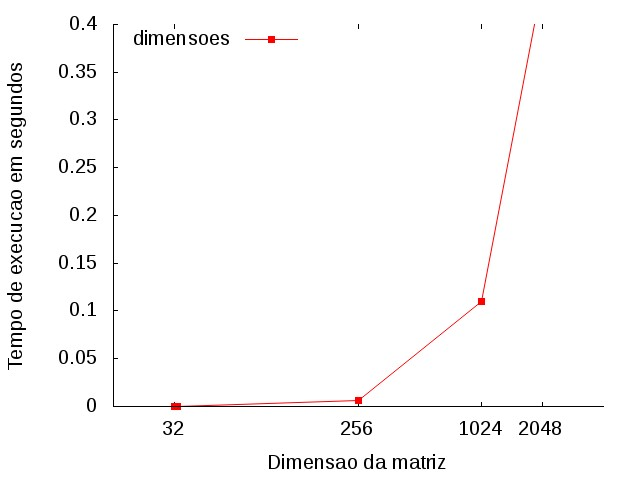
\includegraphics[width=100mm]{img/execucoes.jpg} \end{center}
\caption{Tempo de execução por dimensão da matriz}\label{fig:execucao}
\end{figure}

Em teoria, as execuções do gradSolver com matrizes de dimensões que não são
potência de 2 seriam ligeiramente melhores, por causa de um melhor uso da
associatividade da cache. Porém, isso não pode ser verificado nas execuções para
os tamanhos de cache exibidos acima. Uma melhor visualização dos tempos de
execução pode ser observado na tabela~\ref{fig:tabelaExecucoes}, onde a primeira
coluna são as dimensões da matriz e a segunda os tempos de execução de 50
iterações do método do gradiente em segundos.

\begin{figure}[htb]
\begin{tt}\noindent
    32      0.00014233589172363\\
    33      0.00027585029602051\\
    256     0.00672078132629395\\
    257     0.00610208511352539\\
    1024    0.10956859588623047\\
    1025    0.10990786552429199\\
    2048    0.43970751762390137\\
    2049    0.43948912620544434\\
\end{tt}\caption{Tempo de execução por dimensão da matriz}\label{fig:tabelaExecucoes}
\end{figure}

\section{Análise dos cálculos do fator lambda e resíduo}\label{sec:lambdaResiduo}

\subsection{Medidas de operações em ponto flutuante, memória utilizada e cache
misses}\label{sec:FlopsMemCache}

Utilizando a ferramenta likwid-perfctr, foi possível obter informações nos
trechos de código referentes ao cálculo do fator lambda e do resíduo sobre
memória, cache e operações em ponto flutuante de dupla precisão.

Nos gráficos a seguir, as linhas pretas representam a compilação normal e a
vermelha a compilação otimizada com -O3.

Nos gráficos nas figuras~\ref{fig:cacheLambda} e ~\ref{fig:cacheResidue} podem
ser observadas o total de faltas na cache para uma iteração das funções Lambda
e Resíduo.

\begin{figure} \begin{center}
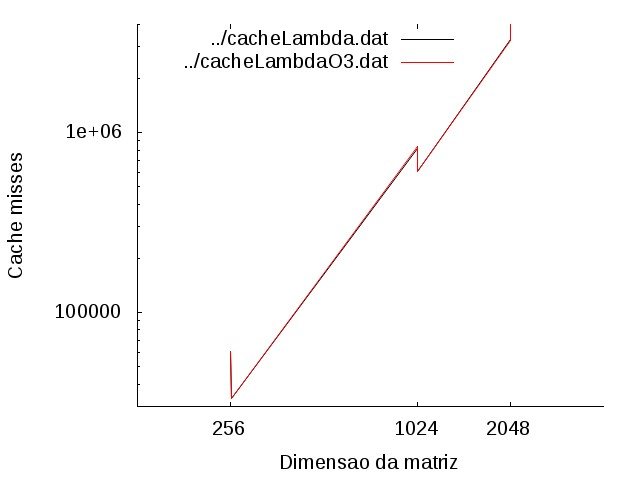
\includegraphics[width=100mm]{img/cacheMissLambda.jpg} \end{center}
\caption{Taxa de falta na cache na função lambda por dimensão da matriz}\label{fig:cacheLambda}
\end{figure}

\begin{figure} \begin{center}
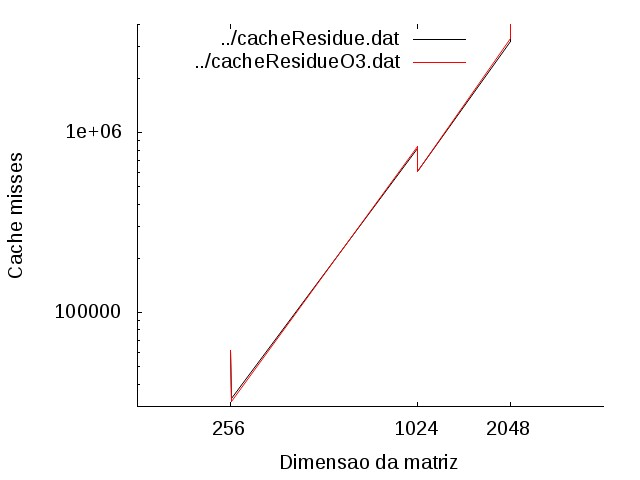
\includegraphics[width=100mm]{img/cacheMissResidue.jpg} \end{center}
\caption{Taxa de falta na cache na função de resíduo por dimensão da matriz}\label{fig:cacheResidue}
\end{figure}

Explicação cache... %FIXME

\clearpage

Já nas figuras~\ref{fig:memLambda} e ~\ref{fig:memResidue}, estão descritas
a quantidade de MBytes/s por dimensão da matriz utilizadas em uma iteração das
funções de cálculo de lambda e resíduo.

\begin{figure}[htb] \begin{center}
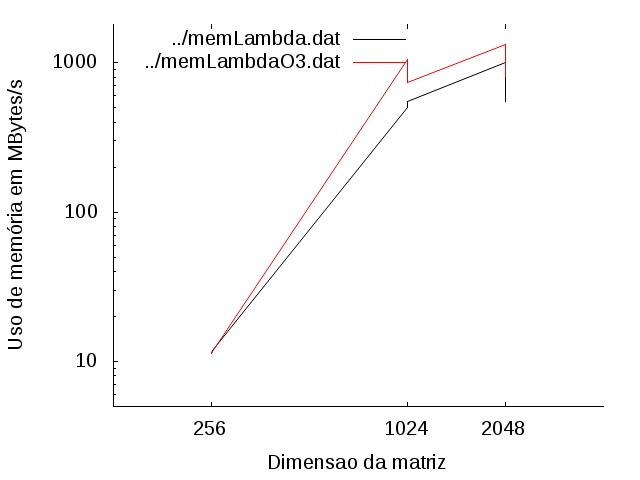
\includegraphics[width=100mm]{img/memLambda.jpg} \end{center}
\caption{Uso de memória em MBytes/s por dimensão da matriz}\label{fig:memLambda}
\end{figure}

\begin{figure}[htb] \begin{center}
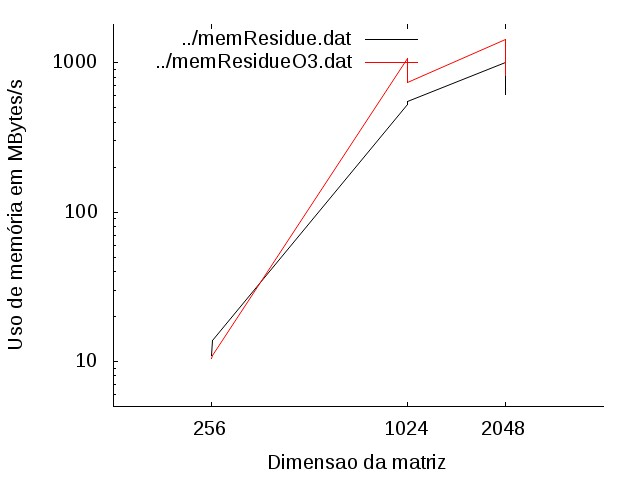
\includegraphics[width=100mm]{img/memResidue.jpg} \end{center}
\caption{Uso de memória em MBytes/s por dimensão da matriz}\label{fig:memResidue}
\end{figure}

A vazão de memória aumenta nas versões otimizadas, pois como várias partes da
memória são acessadas ao mesmo tempo através da vetorização, as operações em
ponto flutuante são efetuadas mais rapidamente.

\clearpage

E por fim, nas figuras~\ref{fig:flopsLambda} e ~\ref{fig:flopsResidue}
encontram-se a quantidade de MFlops/s em relação às dimensões da matriz para
uma iteração dos cálculos de lambda e resíduo.

\begin{figure}[htb] \begin{center}
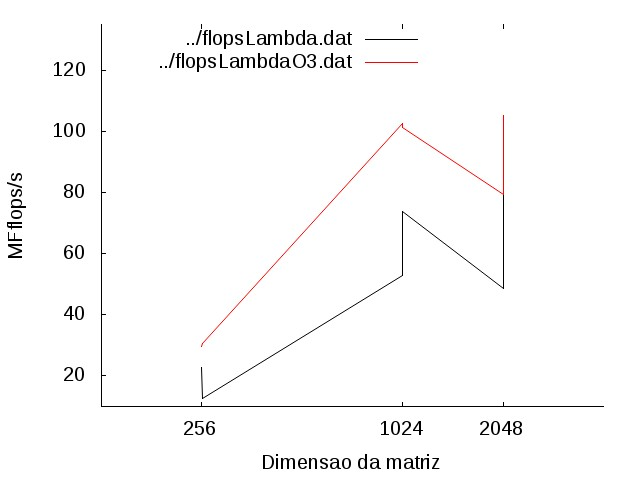
\includegraphics[width=100mm]{img/flopsLambda.jpg} \end{center}
\caption{MFlops/s por dimensão da matriz no cálculo de lambda}\label{fig:flopsLambda}
\end{figure}

\begin{figure}[htb] \begin{center}
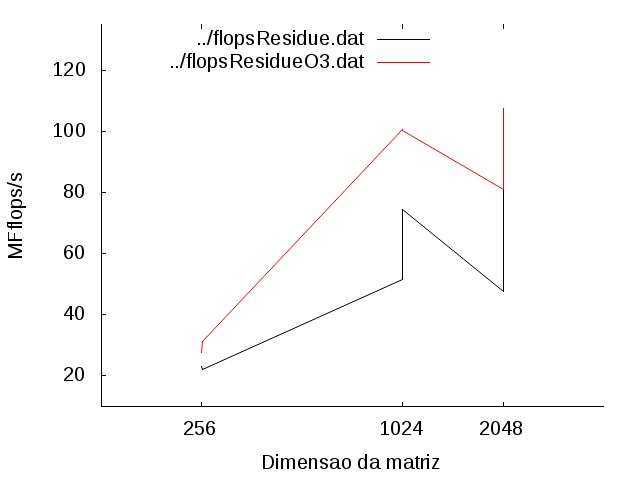
\includegraphics[width=100mm]{img/flopsResidue.jpg} \end{center}
\caption{MFlops/s por dimensão da matriz no cálculo do resíduo}\label{fig:flopsResidue}
\end{figure}

O número de operações em ponto flutuante por segundo também aumenta a medida
que o n aumenta pois há mais operações a serem feitas em menos tempo. Porém,
quando n alcança um certo ponto, o número de flops diminui, já que o
processador só consegue fazer um determinado número de operações em um dado
tempo, e a partir daí as requisições ao processador começam a ter que entrar em
fila e a latência do processador passa a ser um problema. A otimização não
ajuda muito nesse aspecto, pois é uma limitação de hardware.

\clearpage

\subsection{Melhoria no código}\label{sec:melhoria}

Como melhoria do código foi realizado um merge dos laços da multiplicação de
matrizes, e duas multiplicações de vetores, de forma que onde antes se tinha
$2n^2 + 4n$ flops dividos em vários laços para o cálculo da função lambda,
agora as operações de vetores são realizadas dentro do laço da multiplicação de
matrizes, de forma a aproveitar melhor o tempo do processador, o que resulta
numa melhor vazão de MFlops/s.

O gráfico~\ref{fig:compExec} traça uma comparação das compilações normal, com
otimização -O3 e com a melhoria do código para 50 iterações.

\begin{figure}[htb] \begin{center}
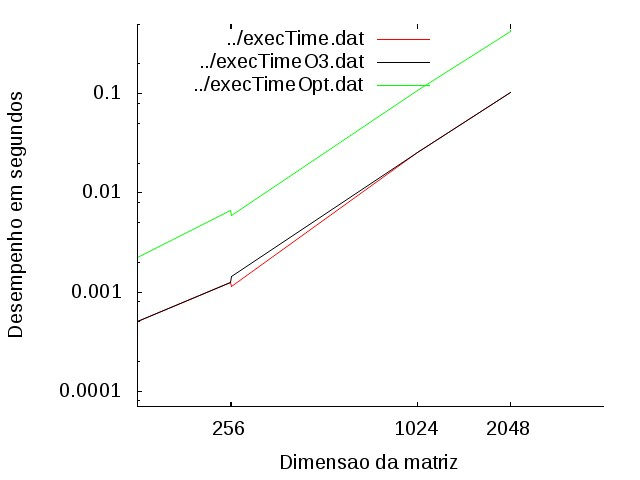
\includegraphics[width=100mm]{img/compExec.jpg} \end{center}
\caption{Desempenho em segundos para compilações normal, com -O3 e com código
otimizado}\label{fig:compExec} \end{figure}

A linha verde representa código com melhoria na função lambda, a vermelha
representa código normal e a linha preta código compilado com a flag de
otimização -O3.

\clearpage

\subsection{Total de operações em ponto flutuante de dupla precisão}\label{sec:flopOp}

Na função multMat, há duas operações em ponto flutuante dentro de dois laços
aninhados, e como as duas operações são uma soma e multiplicação juntas,
conta-se apenas uma operação. Na função linear multVet, há duas operações de
doubles dentro de apenas um laço. Como a função lambda utiliza duas vezes a
função multVet e uma vez a função multMat, a funçao que descreve flops em função
de n é dada por, aproximadamente, $f(n) = 2n^2 + 4n$. Esse valor pode variar com
as otimizações introduzidas pelo compilador.

Para obter esses valores, se utiliza o likwid-perfctr medindo o grupo FLOPS\_DP.
Basta multiplicar o valor em MFlops/s pelo tempo em segundos e então por
$2^{20}$. Assim se obtém o total absoluto de flops utilizados por trecho de
código.

Não foi possível fazer um casamento da complexidade em função da dimensão da
matriz com a conta que se faz com os valores do likwid, pois saída do
likwid-perfctr para FLOPS\_DP sofre muitas variações. Aí seria necessário ler a
documentação da ferramenta  para descobrir se o programa pega os valores por
amostragem de código em execução. Assumindo isso, os valores ficariam mais
próximos aos reais a partir de uma amostragem maior de código, e no caso
apresentado, a medição leva em conta apenas uma iteração do cálculo do lambda.

O mesmo vale para o cálculo do resíduo, que é descrito pela função $f(n) =
2n^2$.

\subsection{Utilização de memória}\label{sec:utilizacaoMemoria}

Nos gráficos~\ref{fig:memLambda} e ~\ref{fig:memResidue} percebe-se que o uso de
memória aumenta em função de N, sendo N a dimensão da matriz de entrada do
gradSolver. Na função lambda, há acessos de memória nas funções de multiplicação
de matrizes e na de vetores, multMat e multVet. Na multMat existem dois laços
aninhados contendo 3 acessos à memória, e na função multVet há 2 acessos à
memória e a mesma é invocada duas vezes. Juntando tudo isso, a função lambda
utiliza $f(n) = 3n^2 + 4n$ doubles de memória, lembrando que cada double possui
8 bytes.

Na mesma linha de raciocínio, a quantidade de memória utilizada pela função de
resíduo é dada por $f(n) = 5n^2$ doubles.

Para verificar os resultados, o mesmo raciocínio feito para descobrir a
quantidade de flops num trecho vale: multiplica-se MBytes/s pelo tempo de
execução, ambas informações coletadas do likwid-perfctr aplicado ao grupo MEM, e
então por $2^{20}$ para se obter a quantia em bytes utilizada pela função.

\end{document}
